\documentclass{article}

\usepackage{amsmath}
\usepackage{tikz}
\usepackage{multicol}
\usepackage{hyperref}
\usepackage{siunitx}


\title{EAS596 \\ Homework 1}
\date{08-30-2018}
\author{Abhishek Kumar\\Instructor : Prof. David Salac}

\begin{document}

\maketitle

\pagenumbering{arabic}
\textbf{1.} In the xy plane, mark all nine of these linear combinations:

\begin{align*}
    y &= c\begin{bmatrix}
           2 \\
           1 \\
         \end{bmatrix}+
         d\begin{bmatrix}
         0\\
         1\\
         \end{bmatrix} \quad with\quad c = 0,1,2 \quad \textrm{and} \quad d = 0,1,2
\end{align*}

\textbf{Solution :}\\
\begin{align*}
y &= \begin{bmatrix}
           2c \\
           c+d \\
         \end{bmatrix}
\end{align*}




\textbf{(a) When c,d = 0,0}
\begin{align*}
y &= \begin{bmatrix}
           2c \\
           c+d \\
         \end{bmatrix} = \begin{bmatrix}
           0 \\
           0 \\
         \end{bmatrix}
\end{align*}
\begin{center}
\begin{tikzpicture}
\draw[step=1cm, gray, very thin] (-1.9,-0.9) grid (2.9,2.9);
\draw[->,ultra thick](0,0) -- (0,0);
\foreach \x in {0,1,2}
    \draw (\x cm,1pt) -- (\x cm,-1pt) node[anchor=north] {$\x$};
\foreach \y in {1,2}
    \draw (1pt,\y cm) -- (-1pt,\y cm) node[anchor=east] {$\y$};
\end{tikzpicture}
\end{center}


\textbf{(b) When c,d = 0,1}
\begin{align*}
y &= \begin{bmatrix}
           2c \\
           c+d \\
         \end{bmatrix}= \begin{bmatrix}
           0 \\
           1 \\
         \end{bmatrix}
\end{align*}
\begin{center}
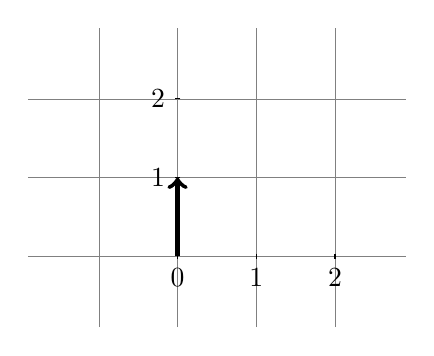
\begin{tikzpicture}
\draw[step=1cm, gray, very thin] (-1.9,-0.9) grid (2.9,2.9);
\draw[->,ultra thick](0,0) -- (0,1);
\foreach \x in {0,1,2}
    \draw (\x cm,1pt) -- (\x cm,-1pt) node[anchor=north] {$\x$};
\foreach \y in {1,2}
    \draw (1pt,\y cm) -- (-1pt,\y cm) node[anchor=east] {$\y$};
\end{tikzpicture}
\end{center}


\textbf{(c) When c,d = 0,2}
\begin{align*}
y &= \begin{bmatrix}
           2c \\
           c+d \\
         \end{bmatrix}= \begin{bmatrix}
           0 \\
           2 \\
         \end{bmatrix}
\end{align*}
\begin{center}
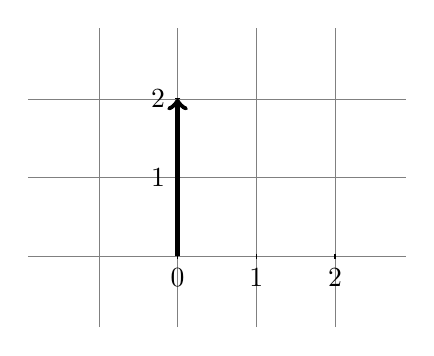
\begin{tikzpicture}
\draw[->,ultra thick](0,0) -- (0,2);\draw[step=1cm, gray, very thin] (-1.9,-0.9) grid (2.9,2.9);
\draw[->,ultra thick](0,0) -- (0,2);
\foreach \x in {0,1,2}
    \draw (\x cm,1pt) -- (\x cm,-1pt) node[anchor=north] {$\x$};
\foreach \y in {1,2}
    \draw (1pt,\y cm) -- (-1pt,\y cm) node[anchor=east] {$\y$};
\end{tikzpicture}
\end{center}


\textbf{(d) When c,d = 1,0}
\begin{align*}
y &= \begin{bmatrix}
           2c \\
           c+d \\
         \end{bmatrix}= \begin{bmatrix}
           2 \\
           1 \\
         \end{bmatrix}
\end{align*}
\begin{center}
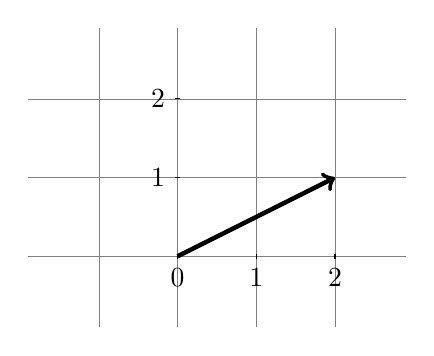
\begin{tikzpicture}[scale=1]
\draw[step=1cm, gray, very thin] (-1.9,-0.9) grid (2.9,2.9);
\draw[->,ultra thick](0,0) -- (2,1);
\foreach \x in {0,1,2}
    \draw (\x cm,1pt) -- (\x cm,-1pt) node[anchor=north] {$\x$};
\foreach \y in {1,2}
    \draw (1pt,\y cm) -- (-1pt,\y cm) node[anchor=east] {$\y$};
\end{tikzpicture}
\end{center}

\textbf{(e) When c,d = 1,1}
\begin{align*}
y &= \begin{bmatrix}
           2c \\
           c+d \\
         \end{bmatrix}= \begin{bmatrix}
           2 \\
           2 \\
         \end{bmatrix}
\end{align*}
\begin{center}
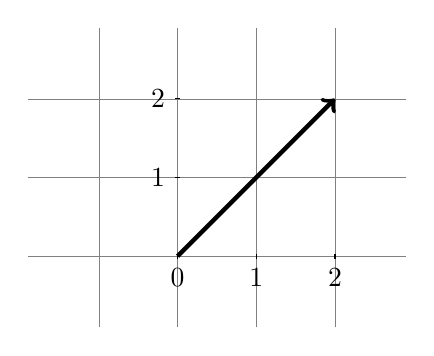
\begin{tikzpicture}[scale=1]
\draw[step=1cm, gray, very thin] (-1.9,-0.9) grid (2.9,2.9);
\draw[->,ultra thick](0,0) -- (2,2);
\foreach \x in {0,1,2}
    \draw (\x cm,1pt) -- (\x cm,-1pt) node[anchor=north] {$\x$};
\foreach \y in {1,2}
    \draw (1pt,\y cm) -- (-1pt,\y cm) node[anchor=east] {$\y$};
\end{tikzpicture}
\end{center}

\textbf{(f) When c,d = 1,2}
\begin{align*}
y &= \begin{bmatrix}
           2c \\
           c+d \\
         \end{bmatrix}= \begin{bmatrix}
           2 \\
           3 \\
         \end{bmatrix}
\end{align*}
\begin{center}
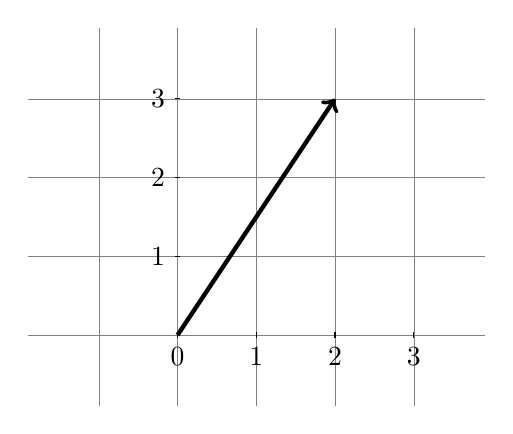
\begin{tikzpicture}[scale=1]
\draw[step=1cm, gray, very thin] (-1.9,-0.9) grid (3.9,3.9);
\draw[->,ultra thick](0,0) -- (2,3);
\foreach \x in {0,1,2,3}
    \draw (\x cm,1pt) -- (\x cm,-1pt) node[anchor=north] {$\x$};
\foreach \y in {1,2,3}
    \draw (1pt,\y cm) -- (-1pt,\y cm) node[anchor=east] {$\y$};
\end{tikzpicture}
\end{center}

\textbf{(g) When c,d = 2,0}
\begin{align*}
y &= \begin{bmatrix}
           2c \\
           c+d \\
         \end{bmatrix}= \begin{bmatrix}
           4 \\
           2 \\
         \end{bmatrix}
\end{align*}
\begin{center}
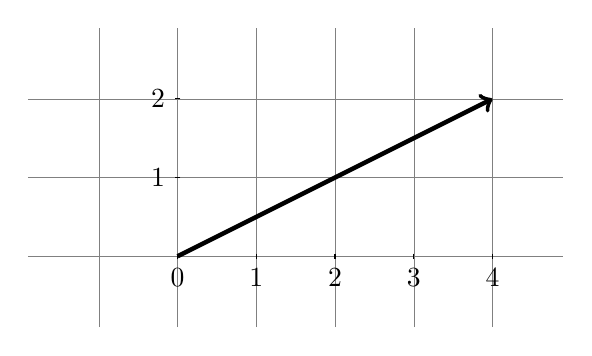
\begin{tikzpicture}[scale=1]
\draw[step=1cm, gray, very thin] (-1.9,-0.9) grid (4.9,2.9);
\draw[->,ultra thick](0,0) -- (4,2);
\foreach \x in {0,1,2,3,4}
    \draw (\x cm,1pt) -- (\x cm,-1pt) node[anchor=north] {$\x$};
\foreach \y in {1,2}
    \draw (1pt,\y cm) -- (-1pt,\y cm) node[anchor=east] {$\y$};
\end{tikzpicture}
\end{center}

\textbf{(h) When c,d = 2,1}
\begin{align*}
y &= \begin{bmatrix}
           2c \\
           c+d \\
         \end{bmatrix}= \begin{bmatrix}
           4 \\
           3 \\
         \end{bmatrix}
\end{align*}
\begin{center}
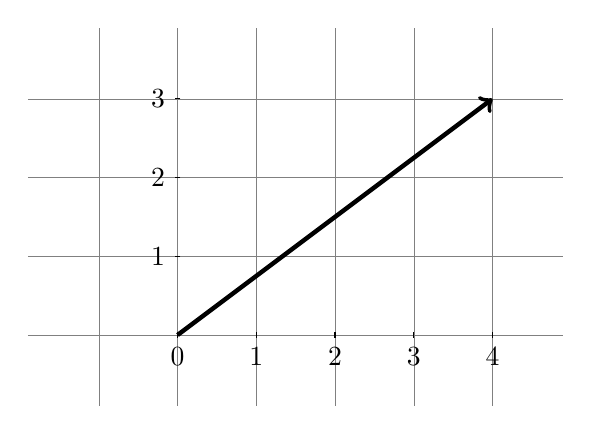
\begin{tikzpicture}[scale=1]
\draw[step=1cm, gray, very thin] (-1.9,-0.9) grid (4.9,3.9);
\draw[->,ultra thick](0,0) -- (4,3);
\foreach \x in {0,1,2,3,4}
    \draw (\x cm,1pt) -- (\x cm,-1pt) node[anchor=north] {$\x$};
\foreach \y in {1,2,3}
    \draw (1pt,\y cm) -- (-1pt,\y cm) node[anchor=east] {$\y$};
\end{tikzpicture}
\end{center}

\textbf{(i) When c,d = 2,2}
\begin{align*}
y &= \begin{bmatrix}
           2c \\
           c+d \\
         \end{bmatrix}= \begin{bmatrix}
           4 \\
           4 \\
         \end{bmatrix}
\end{align*}
\begin{center}
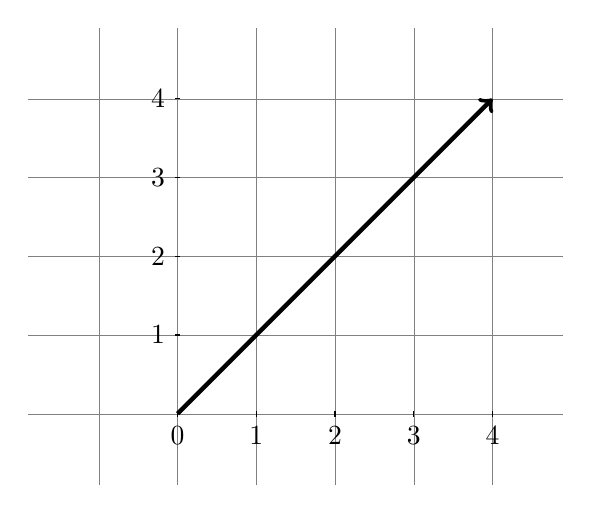
\begin{tikzpicture}[scale=1]
\draw[step=1cm, gray, very thin] (-1.9,-0.9) grid (4.9,4.9);
\draw[->,ultra thick](0,0) -- (4,4);
\foreach \x in {0,1,2,3,4}
    \draw (\x cm,1pt) -- (\x cm,-1pt) node[anchor=north] {$\x$};
\foreach \y in {1,2,3,4}
    \draw (1pt,\y cm) -- (-1pt,\y cm) node[anchor=east] {$\y$};
\end{tikzpicture}\\
\end{center}

\textbf{2. (a)} Find vector $v$ and $w$ so that $v+w=(4,5,6)$ and $v-w=(2,5,8)$.
\textbf{Solution:} We have
\begin{align}
   v+w &= (4,5,6) \\
v-w &= (2,5,8)
\end{align}
Adding (1) and (2), we get
\begin{equation*}
   2v = \left(4+2, 5+5, 6+8\right) = \left(6, 10, 14\right)
\end{equation*}
\begin{equation}
\implies   v = \left(\frac{6}{2}, \frac{10}{2}, \frac{14}{2}\right)\\
\implies v = \left(3, 5, 7\right)
\end{equation}

Now subtracting (2) from (1), we get
\begin{align*}
   (v+w)-(v-w) &= \left(4, 5, 6\right) - \left(2, 5, 8\right)\\
\implies 2w &= (2,0,-2)\\
\implies w &= (1,0,-1)
\end{align*}\\


\textbf{2. (b)} This is a equation with \textbf{$2$} unknown numbers and an equal number of equations to find those numbers.\\This answer is assuming just vectors as unknown but if we solve it assuming variables for each elements of the vectors $v\, and\, w$, we would get 6 unknowns with 6 equations.\\

\textbf{3. (a)} Find unit vectors $u\textsubscript{1}$  and  $u\textsubscript{2}$ in the directions of $v = (3,1)$ and $w =(2,1,2)$. \\
\textbf{Solution:} 
A unit vector in the direction of $u\textsubscript{1}$ is $\left(\frac{u\textsubscript{1}}{\lVert u\textsubscript{1}\rVert }\right) = \left(\frac{(3,1)}{\sqrt{3^2+1^2}}\right) = \left(\frac{3}{\sqrt{10}},\frac{1}{\sqrt{10}}\right)$\\ \\
And a unit vector in the direction of $u\textsubscript{2}$ is $\left(\frac{u\textsubscript{2}}{\lVert u\textsubscript{2}\rVert }\right) = \left(\frac{(2,1,2)}{\sqrt{2^2+1^2+2^2}}\right) = \left(\frac{2}{3},\frac{1}{3},\frac{2}{3}\right)$\\ \\
\\
\textbf{3. (b)} Find unit vectors $U\textsubscript{1}$ and $U\textsubscript{2}$ that are perpendicular to $u\textsubscript{1}$  and  $u\textsubscript{2}$.
\textbf{Solution:} Let $U\textsubscript{1}=(a,b)$ be the unit vector perpendicular to $u\textsubscript{1}$. So we have 
\begin{align}
\lVert (a,b)\rVert = 1 \implies a^2+b^2&=1
\end{align}
\begin{align*}
and, (a,b)\boldsymbol{\cdot}(\left(\frac{3}{\sqrt{10}},\frac{1}{\sqrt{10}}\right))&=\lVert (a,b)\rVert * \lVert (\left(\frac{3}{\sqrt{10}},\frac{1}{\sqrt{10}}\right))\rVert \cos\theta \\
\cos\theta&= 0 \quad because\, \theta =\ang{90}
\end{align*}
\begin{align}
\implies 3a+b=0  \implies b= -3a
\end{align}
Solving equation (4) and (5), we get $a = \pm(\frac{1}{\sqrt{10}})\, and \, b=\mp\left(\frac{3}{\sqrt{10}}\right) $\\
So $U\textsubscript{1}=(\frac{1}{\sqrt{10}},-\frac{3}{\sqrt{10}})$\\

Now, let $U\textsubscript{2}=(x,y,z)$ be the unit vector perpendicular to $u\textsubscript{2}$. So let's can find a vector in the x-y plane which is perpendicular to $u\textsubscript{2}$. Let z = 0
\begin{align}
\lVert (x,y,z)\rVert = 1 \implies x^2+y^2+z^2&=1 \implies x^2+y^2 = 1
\end{align}
\begin{align}
and, (x,y,z)\boldsymbol{\cdot}(1,0.5,1)&=0 \implies x+0.5y = 0
\end{align}
Solving equation (6) and (7), we get $x = \pm(\frac{1}{\sqrt{5}})\, and \, b=\mp\left(\frac{2}{\sqrt{5}}\right) $\\
So $U\textsubscript{2}=(\frac{1}{\sqrt{5}},-\frac{2}{\sqrt{5}},0)$\\ \\

\textbf{4. (a)} If $\lVert v \rVert = 5$ and $\lVert w \rVert = 3$, what are the smallest and the largest values of $\lVert v-w \rVert $\\
\textbf{Solution:} Using law of cosines we have
\begin{align*}
{\lVert v-w \rVert}^2 = {\lVert v \rVert} ^2 + {\lVert w \rVert} ^2 - 2*{\lVert v \rVert}*{\lVert w \rVert}\cos\theta
\end{align*}
Plugging in the values we get,
${\lVert v-w \rVert} = \sqrt{5^2+3^2-2*5*3\cos\theta}$\\
So, the largest value of ${\lVert v-w \rVert}$ will be when $\cos\theta$ is -1 and smallest when $\cos\theta$=1. Therefore the largest value is $\sqrt{5^2+3^2+2*5*3} = \sqrt{64} = 8$. And the smallest value is $\sqrt{5^2+3^2-2*5*3} = \sqrt{4} =2 $\\


\textbf{4. (b)}What are the smallest and largest values of $v\boldsymbol{\cdot}w$?\\
\textbf{Solution:} We know that $v\boldsymbol{\cdot}w = {\lVert v \rVert}{\lVert w \rVert}\cos\theta$
$\implies v\boldsymbol{\cdot}w = 15\cos\theta$\\
The maximum and minimum values of $\cos\theta$ is 1 and -1.
So the maximum and minimum values of $v\boldsymbol{\cdot}w$ is 15 and -15 respectively.\\

\textbf{5.} Consider a parallelogram with sides given by $v$ and $w$. Show that ${\lVert v+w \rVert}^2+{\lVert v-w \rVert}^2 = 2{\lVert v\rVert}^2+2{\lVert w \rVert}^2$.\\
\textbf{Solution:} \\
Using law of cosines we can write\\
${\lVert v+w \rVert}^2+{\lVert v-w \rVert}^2 = ({\lVert v\rVert}^2+{\lVert w \rVert}^2+2{\lVert v \rVert}{\lVert w \rVert}\cos\theta)+({\lVert v\rVert}^2+{\lVert w \rVert}^2-2{\lVert v \rVert}{\lVert w \rVert}\cos\theta)$\\
$\implies {\lVert v+w \rVert}^2+{\lVert v-w \rVert}^2 = 2{\lVert v\rVert}^2+2{\lVert w \rVert}^2$\\

\textbf{6.} Find a combination $x\textsubscript{1}w\textsubscript{1} + x\textsubscript{2}w\textsubscript{2}+x\textsubscript{3}w\textsubscript{3}$ that gives the zero vector. Are these vectors independent or dependent?
\begin{center}
$w\textsubscript{1} =
\left[
\begin{matrix}
1 \\
2\\
3
\end{matrix}
\right],\,
w\textsubscript{2} =
\left[
\begin{matrix}
4 \\
5\\
6
\end{matrix}
\right],\,
w\textsubscript{3} =
\left[
\begin{matrix}
7 \\
8\\
9
\end{matrix}
\right]
$\\
\end{center}
\textbf{Solution:} \, $x\textsubscript{1}w\textsubscript{1} + x\textsubscript{2}w\textsubscript{2}+x\textsubscript{3}w\textsubscript{3} = x\textsubscript{1}\left[
\begin{matrix}
1 \\
2\\
3
\end{matrix}
\right] + x\textsubscript{2}\left[
\begin{matrix}
4 \\
5\\
6
\end{matrix}
\right] +x\textsubscript{3} \left[
\begin{matrix}
7 \\
8\\
9
\end{matrix}
\right]= \left[
\begin{matrix}
0 \\
0\\
0
\end{matrix}
\right]\\
$
\begin{align}
x\textsubscript{1}+4x\textsubscript{2}+7x\textsubscript{3}=0\\
2x\textsubscript{1}+5x\textsubscript{2}+8x\textsubscript{3}=0\\
3x\textsubscript{1}+6x\textsubscript{2}+9x\textsubscript{3}=0
\end{align}
We see that $w\textsubscript{1}+w\textsubscript{3} = 2w\textsubscript{2}$, which means that these are dependent vectors. It also means that there will be infinitely many solutions to the equations above. So, let's find one of those solutions. \\
(9)-2*(8) gives,\\
\begin{align}
-3x\textsubscript{2}-6x\textsubscript{3}=0
\end{align}
\begin{align*}\implies x\textsubscript{2}=-2x\textsubscript{3}
\end{align*} 
So, if $x\textsubscript{3} =1,\, then\, x\textsubscript{2} = -2,\text{ and putting these values in (8), we get }x\textsubscript{1} =1.\text{ So, one of the value of } (x\textsubscript{1},x\textsubscript{2},x\textsubscript{3})$ is  (1,-2,1) \\ \\
\textbf{7. }Let the following matrices be defined.\\
$\\A = 
\left[
\begin{matrix}
4 &7\\
1&2\\
5&6
\end{matrix}
\right], B = 
\left[
\begin{matrix}
4 &3&7\\
1&2&7\\
2&0&4
\end{matrix}
\right], C = 
\left[
\begin{matrix}
3\\
6\\
1
\end{matrix}
\right], D = 
\left[
\begin{matrix}
9&4 &3&-6\\
2&-1&7&5
\end{matrix}
\right], E = 
\left[
\begin{matrix}
1&5&8\\
7&2&3\\
4&0&6
\end{matrix}
\right],\\ \\ \\F = 
\left[
\begin{matrix}
3&0&1\\
1&7&3\\
\end{matrix}
\right], G = 
\left[
\begin{matrix}
7&6&4
\end{matrix}
\right]\\$\\
Answer the following regarding these matrices:\\ \\
\textbf{(a)} What are the dimensions of the matrices?\\
\textbf{Solution:} dim(A) = (3,2), dim(B)=(3,3), dim(C) = (3,1), dim(D)=(2,4), dim(E)=(3,3), dim(F)=(2,3), dim(G)=(1,3)\\ \\
\textbf{(b)}Identify the square,column and row matrices.\\
\textbf{Solution:} \\
\textbf{Square Matrices} = B,E\\
\textbf{Row Matrices} = G\\
\textbf{Column Matrices} = C\\ \\
\textbf{(c)}What are the values of the elements:\,a\textsubscript{12}, b\textsubscript{23}, d\textsubscript{32}, e\textsubscript{22}, f\textsubscript{12}, g\textsubscript{12}\\
\textbf{Solution:}$\,a\textsubscript{12} = 7, b\textsubscript{23}= 7, d\textsubscript{32} = \text{Does not exist}, e\textsubscript{22} =2, f\textsubscript{12} =0, g\textsubscript{12}=6$\\
\textbf{d} Perform the following operations or, if not well defined, explain why:\\ \\
\textbf{(i)}$ E+B$ = $\left[
\begin{matrix}
5&8&15\\
8&4&10\\
6&0&10
\end{matrix}
\right]$\\ \\
\textbf{(ii)}$A+F$ = Cannot perform operation because for addition the dimensions of both the matrices should match.\\ \\
\textbf{(iii)}B-E = $\left[
\begin{matrix}
3&-2&-1\\
-6&0&4\\
-2&0&-2
\end{matrix}
\right]$ \\ \\


\textbf{(iv)} $A\times B$ = Cannot perform operation as matrix-multiplication needs the inner dimensions of the matrices to be the same, here they are different, 2 and 3 respectively.\\


\textbf{(v)}$B\times A = \left[
\begin{matrix}
54&76\\
41&53\\
28&38
\end{matrix}
\right]$ \\ \\ \\


\textbf{(vi)} ${D}^\top =
\left[
\begin{matrix}
9&2\\
4&-1\\
3&7\\
-6&5
\end{matrix}
\right]$\\ \\ \\
\textbf{(vii)} $E \times B = \left[
\begin{matrix}
25&13&74\\
36&25&75\\
28&12&52
\end{matrix}
\right]$\\ \\ \\
\textbf{(viii)}\, ${C}^\top =\left[
\begin{matrix}
3&6&1
\end{matrix}
\right]$\\ \\
\textbf{(ix)}$A \times C =$ Operation cannot be performed because inner dimension of the matrices E and B does not match.\\ \\
\textbf{(x)} $I \times B = B$. Identity matrix multiplied(cross-product) to any matrix yields the same matrix.\\ \\
\textbf{(xi)} ${E}^\top \times E =
\left[
\begin{matrix}
1&7&4\\
5&2&0\\
8&3&6
\end{matrix}
\right] \times  
\left[
\begin{matrix}
1&5&8\\
7&2&3\\
4&0&6
\end{matrix}
\right] = 
\left[
\begin{matrix}
66&19&53\\
19&29&46\\
53&46&109
\end{matrix}
\right]$\\ \\ \\
\textbf{(xii)} ${C}^\top \times C = \left[
\begin{matrix}
3&6&1
\end{matrix}
\right]\times \left[
\begin{matrix}
3\\
6\\
1
\end{matrix}
\right] = 46$.\\ \\


\textbf{8. }Let the following matrices be defined.\\ \\
$A = 
\left[
\begin{matrix}
5&6&6&8\\
2&2&2&8\\
6&6&2&8\\
2&3&6&7
\end{matrix}
\right], \, B = 
\left[
\begin{matrix}
17&-9&12&16\\
17&8.75&-11.75&-16\\
-4&-2.25&2.75&4\\
1&0.75&-0.75&-1
\end{matrix}
\right], \, C = 
\left[
\begin{matrix}
-17&-9&12&16\\
17&8.75&-11.75&-16\\
-4&-2.25&2.75&4\\
1&0.75&-0.75&-1
\end{matrix}
\right] \, $\\
Which matrix, B or C is an inverse to matrix A?\\ \\
\textbf{Solution:} Inverse of a matrix multiplied to itself yields an identity matrix. So the matrix, which when multiplied with A produces an identity matrix is the inverse of A. Let's see.\\ \\
$A\times B = \left[
\begin{matrix}
5&6&6&8\\
2&2&2&8\\
6&6&2&8\\
2&3&6&7
\end{matrix}
\right] \times\left[
\begin{matrix}
17&-9&12&16\\
17&8.75&-11.75&-16\\
-4&-2.25&2.75&4\\
1&0.75&-0.75&-1
\end{matrix}
\right] = \left[
\begin{matrix}
171&0&0&0\\
68&1&0&0\\
204&0&1&0\\
68&0&0&1
\end{matrix}
\right]\\ \\ \\
A\times C = \left[
\begin{matrix}
5&6&6&8\\
2&2&2&8\\
6&6&2&8\\
2&3&6&7
\end{matrix}
\right] \times\left[
\begin{matrix}
-17&-9&12&16\\
17&8.75&-11.75&-16\\
-4&-2.25&2.75&4\\
1&0.75&-0.75&-1
\end{matrix}
\right] = \left[
\begin{matrix}
1&0&0&0\\
0&1&0&0\\
0&0&1&0\\
0&0&0&1
\end{matrix}
\right]\\$ \\
So, we found that C is the inverse of A.
\end{document}